\scanpage{68}
\begin{center}
U N I V E R S I T E\\
DES SCIENCES ET TECHNIQUES\\
DU LANGUEDOC\\
-{}-{}-{}-{}-{}-{}-{}-{}-{}-{}-{}-\\
Service de la Scolarité\\
MR / GJ\\
Diffusion : Liste A\\
N\textdegree\ :4060
\end{center}
Montpellier, le 28 Juin 1978

\begin{center}
\uline{AVIS DE SOUTENANCE D'UN DIPLOME D'ETUDES SUPERIEURES D'UNIVERSITE}
\end{center}

Le 29 JUIN 1978 à 10 Heures\\
Laboratoire de Monsieur le Professeur HALLE\\
Institut de Botanique\\
Université des Sciences et Techniques du Languedoc,

\uline{Monsieur Ibrahima DIAITE}

soutiendra un Diplôme d'Etudes Supérieures d'Université portant sur le
sujet suivant :

``Ecologie de la forêt de Basse-Casamance''.

\uline{Membres du jury}:

\diagram{\(\begin{array}{ll}
\text{MM. :}&\\
&\text{David W. LEE}\\
&\text{B. SAUGIER}\\
&\text{F. HALLE}
\end{array}\)}

Le Secrétaire Général,

\figure{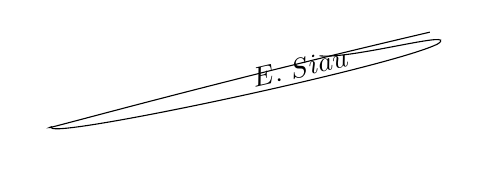
\begin{tikzpicture}
\draw (-2.7,-0.7) .. controls (-3,-0.8) and (-0.9,-0.2) .. (2.1,0.5);
\draw (-2.7,-0.7) .. controls (-2.9,-0.9) and (1.6,0.05) .. (2.2,0.35)
.. controls (2.5,0.55) and (1.1,0.15) .. (0.7,0.2);
\node[rotate=13] at (0.45,0.05) {\(\unsure{E.\ Siau}\)};
\end{tikzpicture}}

\uline{E. SIAU}
\mspage{67}

